\chapter{\ReplicaNextLong{} beállítása és karbantartása}\label{ch:replica-next-setup}

Ez a fejezet a \ReplicaNextLong{} műszeregységre vonatkozik, amelyet a \autoref{fig:next-hardware} ábra mutat.

\begin{figure}[htbp]
    \centering
    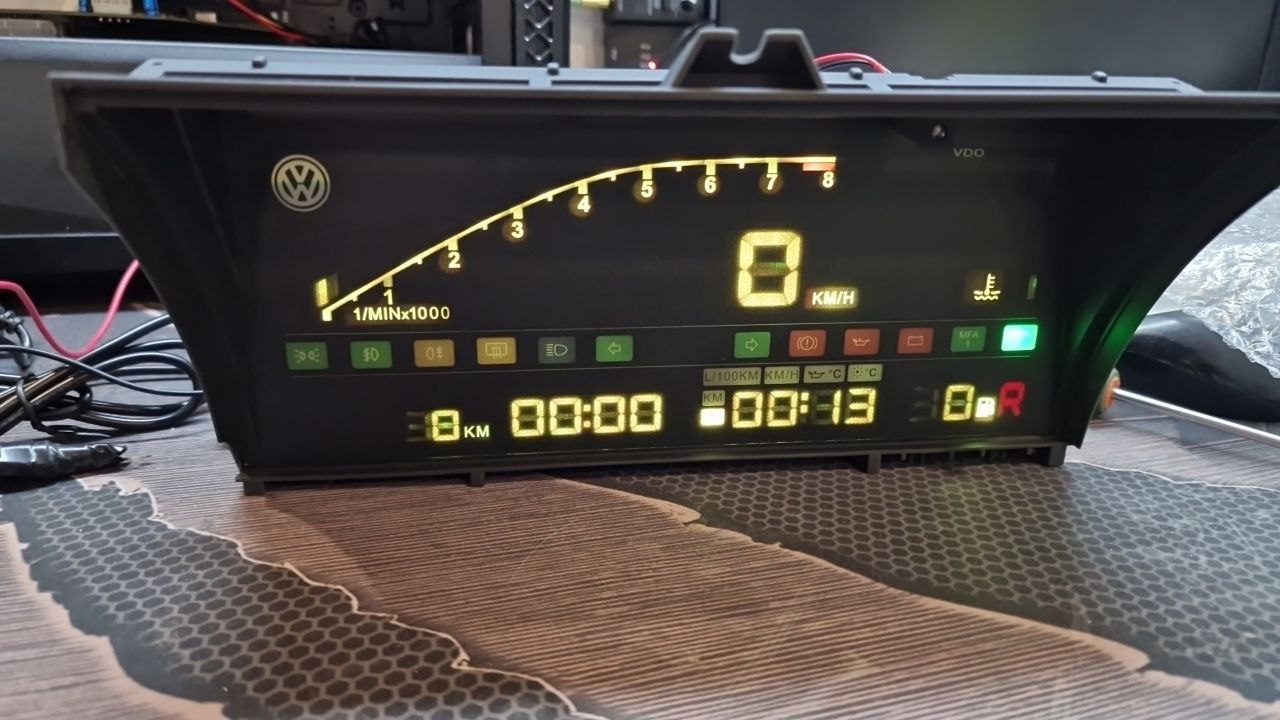
\includegraphics[width=0.6\textwidth]{digifiz_manual/image019.png}
    \caption{\ReplicaNextLong{} műszeregység összeállítás.}
    \label{fig:next-hardware}
\end{figure}

\section{Panelkezelés}
\begin{itemize}
    \item Az UV-nyomott polikarbonát előlapot óvni kell a karcolásoktól és idegen tárgyaktól. Jelentős sérülés esetén PHOL-LABS Kft-től szükséges cserealkatrészt rendelni; ez nem garanciális hiba.
    \item A valós idejű óra a Wi-Fi vezérlőpanelen keresztül állítható, és minden alkalommal visszaáll, ha az állandó tápfeszültséget megszüntetik.
\end{itemize}

\section{Wi-Fi vezérlőportál}
A konfiguráció, az adatgyűjtés és a firmware kezelése a beágyazott webalkalmazáson keresztül történik.
\begin{itemize}
    \item Csatlakozzon a műszerfal Wi-Fi hozzáférési pontjára. Kapcsolja ki a mobiladatot, majd jelentkezzen be a \texttt{Digifiz\_AP} hálózatra (jelszó: \texttt{87654321}); egyes revíziók \texttt{PHOL-LABS2} SSID-t sugároznak ugyanilyen jelszóval.
    \item Az alapértelmezett IP-cím \texttt{192.168.4.1}. Ha a műszerfal más hálózathoz csatlakozik, keressen egy \texttt{.32} végű címet a helyi alhálózaton IP eszközkereső alkalmazással.
    \item A portál öt lapot tartalmaz: \emph{WiFi}, \emph{Control}, \emph{Settings}, \emph{Colors} és \emph{About} (lásd \autoref{fig:next-control-tabs}). A WiFi lap kezeli a hálózati beállításokat és a firmware feltöltést; a Control lap a műszerfal paramétereit módosítja; a Settings lap strukturált szerkesztőt kínál az összes firmware paraméterhez; a Colors lap több szegmensből álló színsémákat kezel; az About lapon a szerzői információk találhatók.
\end{itemize}

\begin{figure}[htbp]
    \centering
    \begin{subfigure}{0.48\textwidth}
        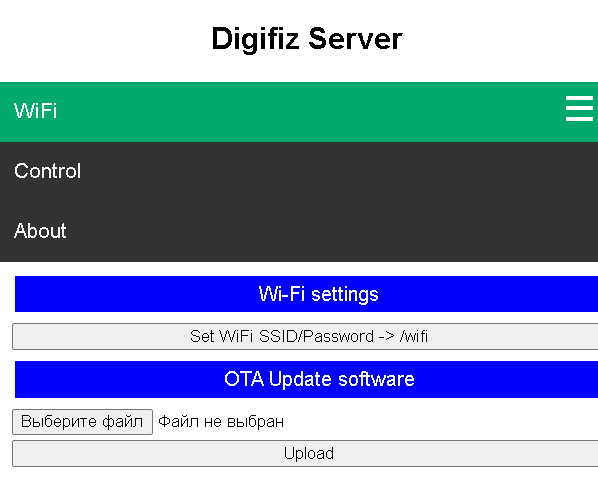
\includegraphics[width=\linewidth]{digifiz_manual/image020.png}
        \caption{A Control lap áttekintése.}
    \end{subfigure}\hfill
    \begin{subfigure}{0.48\textwidth}
        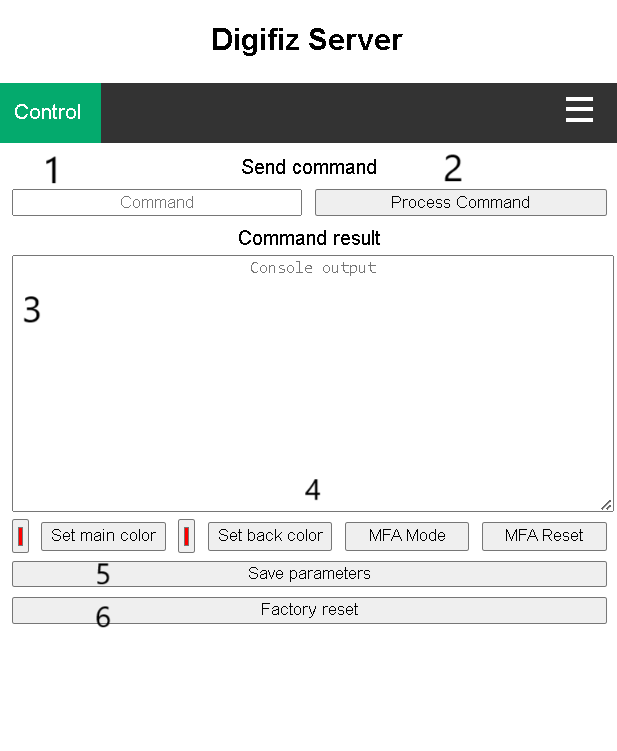
\includegraphics[width=\linewidth]{digifiz_manual/image021.png}
        \caption{Számozott vezérlők és parancsbeviteli mezők.}
    \end{subfigure}
    \caption{\ReplicaNextShort{} Wi-Fi vezérlőfelület.}
    \label{fig:next-control-tabs}
\end{figure}

\section{Parancsbevitel}
A \emph{Control} lap egy parancsbeviteli sort (1), egy \emph{Process} gombot (2), egy eredményablakot (3), gyorsvezérlőket (4), egy \emph{Save} gombot (5) és egy \emph{Reset} gombot (6) tartalmaz. A parancsokat szóközzel elválasztott \verb|<szám> <érték>| párokként kell megadni, kizárólag egész számokkal; írásjelek és idézőjelek nem szükségesek. A \autoref{fig:next-command-example} példa az automatikus fényerő ki- és bekapcsolását szemlélteti.

\begin{figure}[htbp]
    \centering
    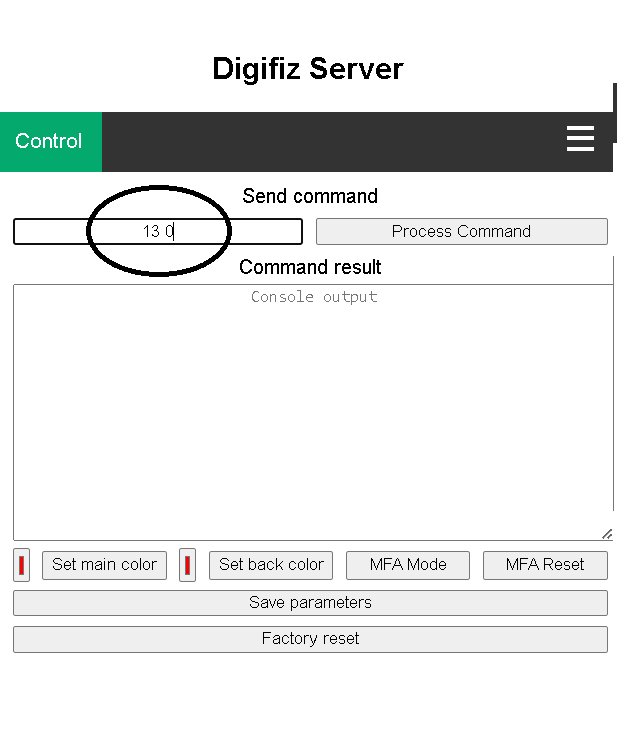
\includegraphics[width=0.55\textwidth]{digifiz_manual/image022.png}
    \caption{Példa parancssorozat az automatikus fényerő kikapcsolására.}
    \label{fig:next-command-example}
\end{figure}

\section{Parancsreferencia}
\begin{table}[htbp]
    \centering
    \caption{A \ReplicaNextShort{} fő konfigurációs parancsai.}
    \label{tbl:next-commands}
    {\scriptsize
    \begin{tblr}{
        colspec = {Q[c,0.14\linewidth] Q[l,0.36\linewidth] Q[l]},
        rowsep = 2pt,
    }
        \toprule
        \textbf{Parancs} & \textbf{Név} & \textbf{Leírás} \\
        \midrule
        22 (vagy 0) & \paramname{PARAMETER\_RPMCOEFFICIENT} & Motorfordulatszám-korrekciós tényező (100--10000). \\
        1  & \paramname{PARAMETER\_SPEEDCOEFFICIENT} & Sebességkorrekciós tényező (10--255). \\
        2  & \paramname{PARAMETER\_COOLANTTHERMISTORB} & Hűtőfolyadék termisztor béta tényező (2000--5000). \\
        3  & \paramname{PARAMETER\_OILTHERMISTORB} & Olaj termisztor béta tényező (2000--5000). \\
        4  & \paramname{PARAMETER\_AIRTHERMISTORB} & Külső levegő termisztor béta tényező (2000--5000). \\
        5  & \paramname{PARAMETER\_TANKMINRESISTANCE} & Minimális üzemanyagszint-ellenállás (0--1000~\ohm). \\
        6  & \paramname{PARAMETER\_TANKMAXRESISTANCE} & Maximális üzemanyagszint-ellenállás (100--1000~\ohm). \\
        7  & \paramname{PARAMETER\_TAU\_COOLANT} & Hűtőfolyadék hőmérséklet szűrőállandó (1--50, nagyobb érték = gyorsabb reakció). \\
        8  & \paramname{PARAMETER\_TAU\_OIL} & Olajhőmérséklet szűrőállandó (1--50). \\
        9  & \paramname{PARAMETER\_TAU\_AIR} & Külső hőmérséklet szűrőállandó (1--50). \\
        10 & \paramname{PARAMETER\_TAU\_TANK} & Üzemanyagszint szűrőállandó (1--50). \\
        11 & \paramname{PARAMETER\_MILEAGE} & Összesített kilométer-számláló (0--999999). \\
        12 & \paramname{PARAMETER\_DAILY\_MILEAGE} & Napi számláló (0--9999). \\
        13 & \paramname{PARAMETER\_AUTO\_BRIGHTNESS} & Automatikus fényerő engedélyezése (1=be, 0=ki). \\
        14 & \paramname{PARAMETER\_BRIGHTNESS\_LEVEL} & Kézi fényerő szint (0--60\%; 60 fölött csökkenti a LED-ek élettartamát). \\
        15 & \paramname{PARAMETER\_TANK\_CAPACITY} & Üzemanyagtartály kapacitása literben (0--99; Golf~2 esetén jellemzően 55~L). \\
        16 & \paramname{PARAMETER\_MFA\_STATE} & Aktív MFA mód (normál esetben hardveres bemenetről vezérelve). \\
        17 & \paramname{PARAMETER\_BUZZER\_OFF} & Hangjelző tiltása (1 letilt, 0 engedélyez; \ReplicaNextShort{} nem tartalmaz hangjelzőt). \\
        18 & \paramname{PARAMETER\_MAX\_RPM} & Fordulatszámmérő skálázás (tipikus 8000, tartomány 4000--16000). \\
        19 & \paramname{PARAMETER\_NORMAL\_RESISTANCE\_COOLANT} & Hűtőfolyadék jeladó ellenállása \SI{25}{\celsius}-on (1000--10000~\ohm). \\
        20 & \paramname{PARAMETER\_NORMAL\_RESISTANCE\_OIL} & Olaj jeladó ellenállása \SI{25}{\celsius}-on (1000--10000~\ohm). \\
        21 & \paramname{PARAMETER\_NORMAL\_RESISTANCE\_AMB} & Külső hőmérséklet jeladó ellenállása \SI{25}{\celsius}-on (1000--10000~\ohm). \\
        23 & \paramname{PARAMETER\_DOT\_OFF} & Órakettőspont viselkedése (0=villog, 1=folyamatos). \\
        24 & \paramname{PARAMETER\_BACKLIGHT\_ON} & Háttérvilágítás engedélyezése tompított fénnyel (\ReplicaNextShort{} nem használja). \\
        25 & \paramname{PARAMETER\_M\_D\_FILTER} & Mediánszűrő állandó (örökölt, általában nem használt). \\
        26 & \paramname{PARAMETER\_COOLANT\_MAX\_R} & Hűtő jeladó küszöb teljes skálához (\SI{100}{\celsius}--\SI{150}{\celsius}). \\
        27 & \paramname{PARAMETER\_COOLANT\_MIN\_R} & Hűtő jeladó küszöb „1~bar” kijelzéshez (\SI{0}{\celsius}--\SI{80}{\celsius}). \\
        31 & \paramname{PARAMETER\_MAINCOLOR\_R} & A felhasználói felület piros komponense (0--255). \\
        32 & \paramname{PARAMETER\_MAINCOLOR\_G} & A felhasználói felület zöld komponense (0--255). \\
        33 & \paramname{PARAMETER\_MAINCOLOR\_B} & A felhasználói felület kék komponense (0--255). \\
        37 & \paramname{PARAMETER\_RPM\_FILTER} & Fordulatszám-szűrő agresszivitás (10--200, nagyobb = gyorsabb reakció). \\
        128 & \paramname{PARAMETER\_READ\_ADDITION} & 128 hozzáadásával bármely parancs aktuális értéke olvasható. \\
        255 & \paramname{PARAMETER\_SET\_HOUR} & Óra beállítása (24 órás formátum). \\
        254 & \paramname{PARAMETER\_SET\_MINUTE} & Perc beállítása. \\
        253 & \paramname{PARAMETER\_RESET\_DAILY\_MILEAGE} & Napi számláló nullázása. \\
        252 & \paramname{PARAMETER\_RESET\_DIGITAL} & Tárolt paraméterek gyári visszaállítása. \\
        \bottomrule
    \end{tblr}}
\end{table}

\section{Alapértelmezett értékek}
\begin{table}[htbp]
    \centering
    \caption{\ReplicaNextShort{} alapbeállítások.}
    \label{tbl:next-defaults}
    {\scriptsize
    \begin{tblr}{
        colspec = {Q[l,0.42\linewidth] Q[c,0.15\linewidth] Q[l]},
        rowsep = 2pt,
    }
        \toprule
        \textbf{Paraméter} & \textbf{Alapérték} & \textbf{Megjegyzés} \\
        \midrule
        \paramname{PARAMETER\_RPMCOEFFICIENT} & 3000 & Tipikus Audi fordulatszám bemenetekhez. \\
        \paramname{PARAMETER\_SPEEDCOEFFICIENT} & 100 & 100~km/h-ra kalibrálva. \\
        \paramname{PARAMETER\_COOLANTTHERMISTORB} & 4000 &  \\
        \paramname{PARAMETER\_OILTHERMISTORB} & 4000 &  \\
        \paramname{PARAMETER\_AIRTHERMISTORB} & 3812 & 3600 a 2. generációs panelekhez. \\
        \paramname{PARAMETER\_TANKMINRESISTANCE} & 35 & \ohm. \\
        \paramname{PARAMETER\_TANKMAXRESISTANCE} & 265 & \ohm. \\
        \paramname{PARAMETER\_TAU\_COOLANT} & 2 & Szűrőállandó. \\
        \paramname{PARAMETER\_TAU\_OIL} & 2 & Szűrőállandó. \\
        \paramname{PARAMETER\_TAU\_AIR} & 2 & Szűrőállandó. \\
        \paramname{PARAMETER\_TAU\_TANK} & 2 & Szűrőállandó. \\
        \paramname{PARAMETER\_MILEAGE} & Járműfüggő & Megőrzi a tárolt futásteljesítményt. \\
        \paramname{PARAMETER\_DAILY\_MILEAGE} & 0 &  \\
        \paramname{PARAMETER\_AUTO\_BRIGHTNESS} & 1 & Engedélyezve. \\
        \paramname{PARAMETER\_BRIGHTNESS\_LEVEL} & 25 & 2. generációs alapérték; az 1/1.5 generáció 7-et vagy 13-at használ. \\
        \paramname{PARAMETER\_TANK\_CAPACITY} & 63 & Liter. \\
        \paramname{PARAMETER\_MFA\_STATE} & 0 & Alapértelmezett MFA oldal. \\
        \paramname{PARAMETER\_BUZZER\_OFF} & 1 & Hangjelző letiltva. \\
        \paramname{PARAMETER\_MAX\_RPM} & 8000 & Fordulatszámmérő skála. \\
        \paramname{PARAMETER\_NORMAL\_RESISTANCE\_COOLANT} & 1000 & \ohm{} \SI{25}{\celsius}-on. \\
        \paramname{PARAMETER\_NORMAL\_RESISTANCE\_OIL} & 1000 & \ohm{} \SI{25}{\celsius}-on. \\
        \paramname{PARAMETER\_NORMAL\_RESISTANCE\_AMB} & 2991 & 500~\ohm{} a 2. generációs érzékelőkhöz. \\
        \paramname{PARAMETER\_DOT\_OFF} & 0 & Villogó kettőspont. \\
        \paramname{PARAMETER\_BACKLIGHT\_ON} & 1 & Háttérvilágítás bekapcsol a tompított fénnyel. \\
        \paramname{PARAMETER\_M\_D\_FILTER} & 65535 & Örökölt mediánszűrő állandó. \\
        \paramname{PARAMETER\_COOLANT\_MAX\_R} & 120 & \si{\celsius}. \\
        \paramname{PARAMETER\_COOLANT\_MIN\_R} & 60 & \si{\celsius}. \\
        \paramname{PARAMETER\_MAINCOLOR\_R} & 180 & Sárgászöld alapérték. \\
        \paramname{PARAMETER\_MAINCOLOR\_G} & 240 & Sárgászöld alapérték. \\
        \paramname{PARAMETER\_MAINCOLOR\_B} & 6 & Sárgászöld alapérték. \\
        \paramname{PARAMETER\_RPM\_FILTER} & 70 & Szűrő reakció. \\
        \paramname{PARAMETER\_UPTIME} & 0 & Futásidő számláló. \\
        \bottomrule
    \end{tblr}}
\end{table}

\section{Paraméterek olvasása és példák}
Paraméter olvasásához adjon 128-at a parancs számához (például a \verb|129 0| a sebességkorrekciós tényezőt jelenti vissza). Gyakori parancsok: az automatikus fényerő kikapcsolása (\verb|13 0|), visszakapcsolása (\verb|13 1|), a sebességkorrekció módosítása (\verb|1 110| 10\%-kal növeli a kijelzett sebességet) és a kilométer-számláló beállítása (\verb|11 123456|). Az óraértékeket a \verb|255 <óra>|, majd a \verb|254 <perc>| parancsokkal lehet megadni. A 31--33 parancsok a felhasználói felület RGB komponenseit állítják.

\section{Szervizparancsok}
Az újabb firmware-verziók emberi olvasású paraméterneveket is elfogadnak, például \verb|PARAMETER_RPMCOEFFICIENT 3000|. A \verb|adc 0| diagnosztikai parancs nyers ADC értékeket jelenít meg a szenzorok hibakereséséhez. A firmware-frissítések vizuális színszabályzókat adnak, ezért rendszeresen frissítsen a \emph{WiFi} lapon, hogy hozzáférjen az új funkciókhoz.

\section{Beállítások lap paraméter szerkesztője}
A \emph{Settings} lap a \autoref{tbl:next-commands} és \autoref{tbl:next-defaults} táblázatokban szereplő listát tükrözi, miközben megjeleníti a tartományokat, leírásokat és adattípusokat. Használja, ha inkább grafikus felületen dolgozna a parancsok beírása helyett.

\begin{enumerate}
    \item Nyomja meg a \emph{Load Parameters} gombot, hogy lekérje az aktuális értékeket a műszerről. A böngésző minden tételt a nevével, aktuális értékével, tippjével és típusával jelenít meg.
    \item Számmezők esetén írja be a kívánt értéket az \emph{New Value} oszlopba. A felület betartatja a \emph{Min} és \emph{Max} oszlopban jelzett megengedett tartományt. A logikai paraméterek jelölőnégyzetként jelennek meg.
    \item Kattintson a \emph{Set} gombra a módosítás azonnali beküldéséhez. A táblázat frissül, és visszaigazolja az új értéket.
    \item Ismételje meg a folyamatot minden módosítandó paraméternél. A végén térjen vissza a \emph{Control} lapra, és nyomja meg a \emph{Save parameters} gombot, hogy a konfiguráció nem felejtő memóriába kerüljön.
\end{enumerate}

A színmunkafolyamat megköveteli, hogy a \emph{Colors} lap használata előtt engedélyezze az egyedi palettákért felelős firmware flaget. Keresse meg a „Custom colour scheme” (a paraméterlistában \verb|PARAMETER_CUSTOM_COLORSCHEME_ENABLE| néven) logikai bejegyzést, pipálja ki, majd nyomja meg a \emph{Set} gombot. A műszer nem fogadja el a szegmensenkénti módosításokat, amíg ez a jelölés nincs aktiválva.

\section{Egyedi színsémák}
A \emph{Colors} lap szegmensalapú szerkesztőt kínál a WS2812 LED háttérvilágításhoz. Minden sor egy tartománylezárást, a hozzárendelt funkcionális területet és a színt vagy az alap színöröklést írja le.

\begin{enumerate}
    \item Nyomja meg a \emph{Load Scheme} gombot az aktuális leképezés beolvasásához. Használja az \emph{Add Segment} gombot, illetve a beépített „+\textuparrow{}” és „+\textdownarrow{}” vezérlőket új tartományok beszúrásához. A legördülő listák a műszer funkcióját választják ki, az alapszín-választó pedig engedi az alap- vagy háttérszínek újrafelhasználását fix RGB érték helyett.
    \item Kattintson a színválasztóra az RGB tónus finomhangolásához, ha a szegmens „Custom” értékre van állítva. A szerkesztő valós időben mutatja a komponensértékeket.
    \item A sorrend nyilakkal rendezze úgy, hogy megfeleljen a fizikai LED-sorrendnek (a szegmenseknek növekvő sorrendben kell maradniuk). A felesleges sorokat távolítsa el a „\texttimes{}” gombbal.
    \item Ha a táblázat a kívánt elrendezést tükrözi, nyomja meg a \emph{Set Scheme} gombot. A böngésző soronként küldi fel a szegmenseket a műszerre.
    \item Azonnal váltson a \emph{Control} lapra, és nyomja meg a \emph{Save parameters} gombot. Ez kötelező lépés — a firmware RAM-ban tárolja a feltöltött szegmenseket, és újraindításkor eldobja őket, ha nem menti.
    \item Opcionálisan exportálja a JSON leírást a \emph{Export to File} funkcióval mentéshez, vagy importáljon korábban elmentett fájlt az \emph{Import from File} segítségével. A \emph{Reset Scheme} gomb megerősítés után visszaállítja a gyári elrendezést.
\end{enumerate}

Ha később kikapcsolja az egyedi színséma flaget a \emph{Settings} lapon, a műszer visszatér a klasszikus, egyszínű módhoz, amelyet a \verb|PARAMETER_MAINCOLOR_R/G/B| parancsok vezérelnek.
